\documentclass[10pt,twocolumn,letterpaper]{article}

\usepackage{cvpr}
\usepackage{times}
\usepackage{epsfig}
\usepackage{graphicx}
\usepackage{amsmath}
\usepackage{amssymb}
\usepackage[numbers,sort,compress]{natbib}
\usepackage{amsfonts}

% Include other packages here, before hyperref.

% If you comment hyperref and then uncomment it, you should delete
% egpaper.aux before re-running latex.  (Or just hit 'q' on the first latex
% run, let it finish, and you should be clear).
\usepackage[breaklinks=true,bookmarks=false]{hyperref}

\cvprfinalcopy % *** Uncomment this line for the final submission

\def\cvprPaperID{****} % *** Enter the CVPR Paper ID here
\def\httilde{\mbox{\tt\raisebox{-.5ex}{\symbol{126}}}}

% Pages are numbered in submission mode, and unnumbered in camera-ready
%\ifcvprfinal\pagestyle{empty}\fi
\setcounter{page}{4321}

\newcommand{\imp}{\vdash_{\cal I}}


%%%%%%%%%%%%%%%%%%%%%%%%%%%%%%%%%%%%%%%%%%
% Enumerate and Itemize modifications
\usepackage{enumitem}
\setlist{topsep=0pt,noitemsep} \setitemize[1]{label=$\circ$}
%%%%%%%%%%%%%%%%%%%%%%%%%%%%%%%%%%%%%%%%%%%


\sloppy
\newcommand{\rtable}[1]{\ensuremath{\mathsf{#1}}}
\newcommand{\ratt}[1]{\ensuremath{\mathit{#1}}}
\newcommand{\at}[1]{\protect\ensuremath{\mathsf{#1}}\xspace}
\newcommand{\myhrule}{\rule[.5pt]{\hsize}{.5pt}}
\newcommand{\oneurl}[1]{\texttt{#1}}
\newcommand{\eat}[1]{}
\newcommand{\stab}{\rule{0pt}{8pt}\\[-1.6ex]}
\newcommand{\sttab}{\rule{0pt}{8pt}\\[-2ex]}
\newcommand{\sstab}{\rule{0pt}{8pt}\\[-2.4ex]}
\newcommand{\tabstrut}{\rule{0pt}{4pt}\vspace{-0.07in}}
\newcommand{\vs}{\vspace{1ex}}
\newcommand{\exa}[2]{{\tt\begin{tabbing}\hspace{#1}\=\+\kill #2\end{tabbing}}}
\newcommand{\ra}{\rightarrow}
\newcommand{\la}{\leftarrow}
\newcommand{\bi}{\begin{itemize}}
\newcommand{\ei}{\end{itemize}}
\newenvironment{tbi}{\begin{itemize}
        \setlength{\topsep}{1.5ex}\setlength{\itemsep}{0ex}}
%\vspace{-0.5ex}}
        {\end{itemize}\vspace{-0.5ex}}
\newenvironment{tbe}{\begin{enumerate}
        \setlength{\topsep}{0ex}\setlength{\itemsep}{0ex}\vspace{0ex}}
        {\end{itemize}\vspace{-1ex}}

\newcommand{\noteqs}[1]{{\color{red}{#1}---QS}}

\newcommand{\mat}[2]{{\begin{tabbing}\hspace{#1}\=\+\kill #2\end{tabbing}}}
\newcommand{\m}{\hspace{0.05in}}
\newcommand{\ls}{\hspace{0.1in}}
\newcommand{\be}{\begin{enumerate}}
\newcommand{\ee}{\end{enumerate}}
\newcommand{\beqn}{\begin{eqnarray*}}
\newcommand{\eeqn}{\end{eqnarray*}}
\newcommand{\card}[1]{\mid\! #1\!\mid}
\newcommand{\fth}{\hfill $\Box$}
\newcommand{\AND}{\displaystyle{\bigwedge_{i=1}^{n}}}
\newcommand{\U}[1]{\displaystyle{\bigcup_{#1}}}
\newcommand{\Sm}[1]{\displaystyle{\sum_{#1}}}
\newcommand{\stitle}[1]{\vspace{1.5ex}\noindent{\bf #1}}
\newcommand{\etitle}[1]{\vspace{0.8ex}\noindent{\em #1}}
\renewcommand{\t}{\tau}
\newcommand{\Inh}[1]{\$#1}
\renewcommand{\r}[1]{{\it rule}(#1)}
\newcommand{\pa}{\parallel}
\newcommand{\LHS}{\kw{{\small LHS}}\xspace}
\newcommand{\RHS}{\kw{RHS}\xspace}
\newcommand{\ie}{\emph{i.e.,}\xspace}
\newcommand{\eg}{\emph{e.g.,}\xspace}
\newcommand{\wrt}{\emph{w.r.t.}\xspace}
\newcommand{\aka}{\emph{a.k.a.}\xspace}
\newcommand{\kwlog}{\emph{w.l.o.g.}\xspace}
%%%%%%%%%%%%%%%%%%%%%%%%%%%%%%%%%%%%%%%%%%%%%%%%%%%%%%%%%%%%%%%%
%                  Relation Algebra operators
%%%%%%%%%%%%%%%%%%%%%%%%%%%%%%%%%%%%%%%%%%%%%%%%%%%%%%%%%%%%%%%%


\newcommand{\RS}{{\small S}\xspace}
\newcommand{\RP}{{\small P}\xspace}
\newcommand{\RJ}{{\sc j}\xspace}
\newcommand{\RC}{{\small C}\xspace}
\newcommand{\RSJ}{{\small SJ}\xspace}
\newcommand{\RSC}{{\small SC}\xspace}
\newcommand{\RSP}{{\small SP}\xspace}
\newcommand{\RPJ}{{\small PJ}\xspace}
\newcommand{\RPC}{{\small PC}\xspace}
\newcommand{\RSPJ}{{\sc spj}\xspace}
\newcommand{\RSPC}{{\small SPC}\xspace}
\newcommand{\RSPJU}{{\sc spju}\xspace}
\newcommand{\RSPCU}{{\small SPCU}\xspace}
\newcommand{\RSPJUN}{{\small SPJU$^N$}\xspace}
\newcommand{\RSPCUN}{{\small SPCU$^N$}\xspace}

%%%%%%%%%%%%%%%%%%%%%%%%%%%%
% operators
%%%%%%%%%%%%%%%%%%%%%%%%%%%%
\DeclareMathOperator*{\argmin}{arg\,min}

%%%%%%%%%%%%%%%%%%%%%%%%%%%%%%%%%%%%%%%%%%%%%%%%%%%%%%%%%%%%%%%%%%%%%%%%%%%%%%
% ALGORITHMS
%%%%%%%%%%%%%%%%%%%%%%%%%%%%%%%%%%%%%%%%%%%%%%%%%%%%%%%%%%%%%%%%%%%%%%%%%%%%%%%
\newcommand{\SELECT}{\mbox{{\bf select}}\ }
\newcommand{\FROM}{\mbox{{\bf from}\ }}
\newcommand{\WHERE}{\mbox{\bf where}\ }
\newcommand{\SUM}{\mbox{{\bf sum}}\ }
\newcommand{\GROUPBY}{\mbox{{\bf group by}}\ }
\newcommand{\HAVING}{\mbox{{\bf having}}\ }
\newcommand{\CASE}{\mbox{{\bf case}}\ }
\newcommand{\END}{\mbox{{\bf end}}\ }
\newcommand{\WHEN}{\mbox{{\bf when}}\ }
\newcommand{\EXISTS}{\mbox{{\bf exists}}\ }
\newcommand{\COUNT}{\mbox{\kw{count}}}
\newcommand{\INSERTINTO}{\mbox{{\bf insert into}}\ }
\newcommand{\UPDATE}{\mbox{{\bf update}}\ }
\newcommand{\SET}{\mbox{{\bf set}}\ }
\newcommand{\IN}{\mbox{{\bf in}}\ }
\newcommand{\If}{\mbox{\bf if}\ }
\newcommand{\Let}{\mbox{\bf let}\ }
\newcommand{\Call}{\mbox{\bf call}\ }
\newcommand{\Then}{\mbox{\bf then}\ }
\newcommand{\To}{\mbox{\bf to}\ }
\newcommand{\Else}{\mbox{\bf else}\ }
\newcommand{\ElseIf}{\mbox{\bf elseif}\ }
\newcommand{\While}{\mbox{\bf while}\ }
\newcommand{\Begin}{\mbox{\bf begin}\ }
\newcommand{\End}{\mbox{\bf end}\ }
\newcommand{\Do}{\mbox{\bf do}\ }
\newcommand{\Downto}{\mbox{\bf downto}\ }
\newcommand{\Repeat}{\mbox{\bf repeat}\ }
\newcommand{\Until}{\mbox{\bf until}\ }
\newcommand{\For}{\mbox{\bf for}\ }
\newcommand{\Each}{\mbox{\bf each}\ }

\newcommand{\ForEach}{\mbox{\bf for each}\ }
\newcommand{\Or}{\mbox{\bf or}\ }
\renewcommand{\And}{\mbox{\bf and}\ }
\newcommand{\Not}{\mbox{\bf not}\ }
\newcommand{\Break}{\mbox{\bf break}\ }
\newcommand{\Continue}{\mbox{\bf continue}\ }
\newcommand{\Return}{\mbox{\bf return}\ }
\newcommand{\Case}{\mbox{\bf case}\ }
\newcommand{\Of}{\mbox{\bf of}\ }
\newcommand{\EndCase}{\mbox{\bf end-case}\ }
\newcommand{\NIL}{\mbox{\em nil}}
\newcommand{\False}{\mbox{\em false}}
\newcommand{\True}{\mbox{\em true}}
\newcommand{\algAND}{{\sc and}\xspace}
\newcommand{\OR}{{\sc or}\xspace}
\newcommand{\NOT}{{\sc not}\xspace}
\newcommand{\kw}[1]{{\ensuremath {\mathsf{#1}}}\xspace}
\newcommand{\Reps}{S}
\newcounter{ccc}
\newcommand{\bcc}{\setcounter{ccc}{1}\theccc.}
\newcommand{\icc}{\addtocounter{ccc}{1}\theccc.}
\newcommand{\checking}{{\mbox{\small\sf Checking}\xspace}}
\newcommand{\preProcessing}{{\mbox{\small\sf preProcessing}\xspace}}
\newcommand{\CFDconsistency}{{\mbox{\small\sf CFD\_Checking}\xspace}}
\newcommand{\MCS} {\kw{MCS}}
\newcommand{\templateDB}{{\mbox{\small\sf templateDB}\xspace}}
\newcommand{\ChaseChecking}{{\mbox{\small\sf RandomChecking}\xspace}}
\newcommand{\chase}{{\mbox{\small\sf Chase}\xspace}}
\newcommand{\SAT}{{\mbox{\small\sf SAT}\xspace}}
\newcommand{\kSAT}{{\mbox{\small 3SAT}\xspace}}
\newcommand{\PropCFDSPC}{\kw{Prop{\small CFD\_SPC}}}
\newcommand{\PropCFDSPCU}{\kw{Prop{\small CFD\_SPCU}}}
\newcommand{\UnionEQs}{\kw{UnionEQs}}
\newcommand{\UnionCFDs}{\kw{UnionCFDs}}
\newcommand{\EQ}{\kw{EQ}}
\newcommand{\eq}{\kw{eq}}
\newcommand{\key}{\kw{key}}
\newcommand{\rep}{\kw{rep}}
\newcommand{\PEQ}{\kw{EQ2CFD}}
\newcommand{\Drop}{\kw{Drop}}
\newcommand{\Res}{\kw{Res}}
\newcommand{\CFD}{{\small CFD}\xspace}
\newcommand{\CFDs}{{\small CFD}{\small s}\xspace}
\newcommand{\CIND}{{\sc cind}\xspace}
\newcommand{\cind}{{\small \sf CIND}}
\newcommand{\cfd}{{\small \sf CFD}}
\newcommand{\CINDp}{{\sc cind}$^+$\xspace}
\newcommand{\CINDn}{{\sc cind}$^-$\xspace}
\newcommand{\CINDs}{{\sc cind}{\small s}\xspace}
\newcommand{\FD}{{\small FD}\xspace}
\newcommand{\FDs}{{\small FD}{\small s}\xspace}
\newcommand{\IND}{{\sc ind}\xspace}
\newcommand{\INDs}{{\sc ind}{\small s}\xspace}
\newcommand{\TGDs}{{\sc tgd}{\small s}\xspace}
\newcommand{\NP}{\kw{NP}}
\newcommand{\DAGs}{{\small DAG}s\xspace}
\newcommand{\NC}{{\sc nc}\xspace}
\newcommand{\coNP}{co{\sc np}\xspace}
\newcommand{\PTIME}{\kw{PTIME}}
\newcommand{\PSPACE}{\kw{PSPACE}}
\newcommand{\EXPTIME}{\kw{EXPTIME}}
\newcommand{\SharpP}{\kw{\#P}}
\newcommand{\NPSPACE}{\kw{NNPSPACE}}
\newcommand{\dom}{\protect\ensuremath{\mathsf{dom}}\xspace}
\newcommand{\atset}{\protect\ensuremath{\mathsf{attr}}\xspace}
\newcommand{\attr}[1]{\protect\ensuremath{\mathsf{#1}}\xspace}
\newcommand{\attrset}{\protect\ensuremath{\mathsf{attr}}\xspace}
\newcommand{\finatset}{\protect\ensuremath{\mathsf{finattr}}\xspace}
\newcommand{\pvar}{\protect\ensuremath{\mathsf{var\%}}\xspace}
\newcommand{\lLHS}{\protect\ensuremath{\mathsf{{\small LHS}}}\xspace}
\newcommand{\RA}{{\small RA}\xspace}
\newcommand{\RBR}{\kw{RBR}}
\newcommand{\SQL}{{\sc sql}\xspace}
\newcommand{\XSLT}{{\sc xslt}\xspace}
\newcommand{\DBMS}{{\sc dbms}\xspace}
\newcommand{\ATG}{{\sc atg}\xspace}
\newcommand{\ATGs}{{\sc atg}{\small s}\xspace}
\newcommand{\EBI}{{\sc ebi}\xspace}
\newcommand{\GO}{{\sc go}\xspace}
\newcommand{\VEC}[1]{{\sc vec}(#1)}
\newcommand{\DAG}{{\small DAG}\xspace}
\newcommand{\XQ}{{\sc xq}\xspace}
\newcommand{\XQwc}{{\sc xq}$^{\scriptscriptstyle[*]}$\xspace}
\newcommand{\XQdes}{{\sc xq}$^{\scriptscriptstyle[//]}$\xspace}
\newcommand{\XQfull}{{\sc xq}$^{\scriptscriptstyle[*,//]}$\xspace}
\newcommand{\vect}[1]{$\langle$ #1 $\rangle$}
\newcommand{\sem}[1]{[\![#1]\!]}
\newcommand{\NN}[2]{#1\sem{#2}}
\newcommand{\e}[2]{{\mathit (#1,#2)}}
\newcommand{\ep}[2]{{\mathit (#1,#2)+}}
\newcommand{\brname}{\ensuremath{{\mathsf{N}}}}
\newcommand{\budrel}[1]{\ensuremath{{\brname_{#1}}}}
\newcommand{\budgen}[2]{\ensuremath{Q^\brname_\e{#1}{#2}}}
\newcommand{\budcut}[2]{\ensuremath{Q_\e{#1}{#2}}}
\newcommand{\R}{{\cal R}}
\newcommand{\A}{{\cal A}}
\newcommand{\Q}{{\cal Q}}
\newcommand{\Y}{{\cal Y}}
\newcommand{\I}{{\cal I}}
\newcommand{\V}{{\cal V}}
\newcommand{\E}{{\cal E}}
\newcommand{\Lq}{{\cal L}}

\newcommand{\precision}{\kw{precs}}
\newcommand{\recall}{\kw{recall}}
\newcommand{\accuracy}{\kw{accuracy}}

\newcommand{\eop}{\hspace*{\fill}\mbox{$\Box$}}     % End of proof
\newcounter{example}%[section]
\renewcommand{\theexample}{\arabic{example}}
\newenvironment{example}{
        \vspace{1.5ex}
        \refstepcounter{example}
        {\noindent\bf Example \theexample:}}{
        \eop\vspace{1.5ex}}
\def\copyrightspace{}
\renewcommand{\ni}{\noindent}
\newcommand{\nthesection}{\arabic{section}}
\newcounter{theorem}
\renewcommand{\thetheorem}{\arabic{theorem}}
\newcounter{prop}
\renewcommand{\theprop}{\arabic{theorem}}
\newcounter{lemma}
\renewcommand{\thelemma}{\arabic{theorem}}
\newcounter{cor}
\renewcommand{\thecor}{\arabic{theorem}}
\newenvironment{theorem}{\begin{em}
        \refstepcounter{theorem}
        {\vspace{1.5ex} \noindent\bf  Theorem  \thetheorem:}}{
        \end{em}\eop\vspace{1.5ex}} %\hspace*{\fill}\vspace*{1ex}}
\newenvironment{conjecture}{\begin{em}
        \refstepcounter{theorem}
        {\vspace{1.5ex} \noindent\bf  Conjecture  \thetheorem:}}{
        \end{em}\eop\vspace{1.5ex}} %\hspace*{\fill}\vspace*{1ex}}
\newenvironment{prop}{\begin{em}
        \refstepcounter{theorem}
        {\vspace{1.5ex}\noindent \bf Proposition \theprop:}}{
        \end{em}\eop\vspace{1.5ex}}%\hspace*{\fill}\vspace*{1ex}}
\newenvironment{lemma}{\begin{em}
        \refstepcounter{theorem}
        {\vspace{1ex}\noindent\bf Lemma \thelemma:}}{
        \end{em}\eop\vspace{1ex}} %\hspace*{\fill}\vspace*{1ex}}
\newenvironment{cor}{\begin{em}
        \refstepcounter{theorem}
        {\vspace{1.5ex}\noindent\bf Corollary \thecor:}}{
        \end{em}\eop\vspace{1.5ex}} %\hspace*{\fill}\vspace*{1ex}}
\newcounter{definition}[section]
\renewcommand{\thedefinition}{\nthesection.\arabic{definition}}
\newenvironment{definition}{
        \vspace{1.5ex}
        \refstepcounter{definition}
        {\noindent\bf Definition {\bf \thedefinition}:}}{\eop\vspace{1.5ex}
}
\newcounter{alg}[section]
\renewcommand{\thealg}{\nthesection.\arabic{alg}}
\newenvironment{alg}[1]{
        \refstepcounter{alg}
        {\vspace{1ex}\noindent\bf Algorithm \thealg:\, #1}}{
        \vspace*{1ex}}
\newcounter{arule}
\renewcommand{\thearule}{\arabic{arule}}
\newenvironment{arule}{
        \vspace{0.6ex}
        \refstepcounter{arule}
        {\noindent \em Rule \thearule:}}{
        }
\newcounter{claim}
\renewcommand{\theclaim}{\arabic{claim}}
\newenvironment{proof}{
        \vspace{1ex}
        {\noindent\bf Proof:}}{\eop\vspace{1ex}}
\newenvironment{proofS}{
        \vspace{1ex}
        {\noindent\bf Proof sketch:\ }}{\eop\vspace{1ex}}

\renewcommand{\texttt}[1]{{\small\textsf{#1}}}

%\newcommand{\revise}[1]{\textcolor{black}{#1}}%blue
\newcommand{\reviseq}[1]{\textcolor{black}{#1}}%green
\newcommand{\changed}[1]{\textcolor{red}{#1}}
\newcommand{\removed}[1]{\textcolor{gray}{#1}}
\newcommand{\note}[1]{\textcolor{blue}{#1}}

\newcommand{\conv}{conv}
%\DeclareMathOperator{\conf}{conf}
%\DeclareMathOperator{\sim}{sim}
\newcommand{\lift}{lift}
\newcommand{\supp}{\kw{supp}}
\newcommand{\join}{Join}
\newcommand{\Union}{\bigcup}
\newcommand{\nfa} {\kw{NFA}}

\newcommand{\tbf}{\textbf{\textcolor[rgb]{1,0,0}{TBF}}\xspace}

\newcommand{\spmine}{\kw{approxDis}}
\newcommand{\incsum}{\kw{incSum}}
\newcommand{\atmine}{\kw{streamDis}}
\newcommand{\patmine}{\kw{paraDis}}
\newcommand{\patnmine}{\kw{paraDisn}}
\newcommand{\pr}{\kw{PRA}}
\newcommand{\sfe}{\kw{SFE}}
\newcommand{\deeppath}{\kw{DeepPath}}

\newcommand{\oprgen}{\kw{OpGen}}
\newcommand{\apn}{\kw{APN}}
\newcommand{\mbs}{\kw{MBS}}
\newcommand{\genprune}{\kw{GenMBS}}%OpGen
\newcommand{\genseed}{\kw{GenPicky}}%OpGen

\newcommand{\pgen}{\kw{sumGen}}
\newcommand{\inctopk}{\kw{incTopk}}
\newcommand{\fmine}{\kw{heuDis}}
\newcommand{\ftopk}{\kw{fastTopk}}
\newcommand{\aff}{\kw{Aff}}
\newcommand{\smatch}{\kw{evalSum}}
\newcommand{\spsel}{\kw{Select}-\kw{Sum}}
\newcommand{\grami}{\kw{GRAMI}}


\newcommand{\swn}{\kw{FastWhyNot}}
\newcommand{\mwn}{\kw{MultiWhyNot}}
\newcommand{\isown}{\kw{ExactWhyNot}}
\newcommand{\misown}{\kw{MultiExactWhyNot}}
\newcommand{\swniso}{\kw{IsoWhyNot}}
\newcommand{\enuwn}{\kw{EnuWhyNot}}

\newcommand{\sw}{\kw{ApproxWhy}}
\newcommand{\msw}{\kw{MultiApproxWhy}}
\newcommand{\misow}{\kw{MultiExactWhy}}
\newcommand{\isow}{\kw{ExactWhy}}
\newcommand{\enuw}{\kw{EnuWhy}}
\newcommand{\swiso}{\kw{IsoWhy}}

\newcommand{\parti}{\kw{Ptn}}
\newcommand{\msg}{\kw{Msg}}
\newcommand{\lscan}{\kw{Lscan}}
\newcommand{\pncons}{\kw{PnCons}}
\newcommand{\assign}{\kw{Assign}}
\newcommand{\leval}{\kw{LocalEval}}
\newcommand{\prcons}{\kw{PrCons}}
\newcommand{\diffc}{\kw{DiffCal}}
\newcommand{\simq}{\kw{Sim_q}}
\newcommand{\simst}{\kw{Sim_{st}}}
\newcommand{\simse}{\kw{Sim_{se}}}
\newcommand{\simr}{\kw{Sim_r}}
\newcommand{\mcs}{\kw{mcs}}

\newcommand{\divsum}{\kw{sumDiv}}
\newcommand{\eetitle}[1]{\vspace{0.8ex}\noindent{\em\underline{#1}}}

\newcommand{\parpgen}{\kw{ParsumGen}}
\newcommand{\pardivsum}{\kw{ParsumDiv}}

\newcommand{\smatchr}{\kw{evalRnd}}
\newcommand{\smatcha}{\kw{evalSum}($\Delta$=0)\xspace}
\newcommand{\smatchi}{\kw{evalGRAMI}}
\newcommand{\smatchno}{\kw{evalNo}}

\newcommand{\yago}{\kw{Yago}}
\newcommand{\dbpedia}{\kw{DBpedia}}
\newcommand{\freebase}{\kw{Freebase}}
\newcommand{\pokec}{\kw{Pokec}}
\newcommand{\amazon}{\kw{Amazon}}
\newcommand{\imdb}{\kw{IMDB}}
%\newcommand{\simk}{$\preceq_d$}
\newcommand{\diff}{\kw{diff}}
\newcommand{\warn}[1]{{\color{red}{#1}}}
\newcommand\addtag{\refstepcounter{equation}\tag{\theequation}}

\newcommand{\spawn}{\kw{Spawn}}

\newcommand{\lvec}{\kw{lvec}}

\newcommand{\rms}{\kw{RMS}}
\newcommand{\rmss}{\kw{RMSs}}

\newcommand{\reduce}{\kw{Reduce}}
\newcommand{\validate}{\kw{Validate}}

\newcommand{\op}{\kw{op}}
\newcommand{\oc}{\kw{oc}}
\newcommand{\avg}{\kw{avg}}
\newcommand{\cl}{\kw{cl}}
\newcommand{\pre}{\kw{guard}}
\newcommand{\ecl}{\kw{\hat{cl}}}
\newcommand{\cost}{\kw{cost}}
\newcommand{\bsm}{\kw{BSM}}

\newcommand{\revise}[1]{{\color{black}{#1}}}
\newcommand{\reviseOne}[1]{{\color{black}{#1}}}
\newcommand{\reviseTwo}[1]{{\color{black}{#1}}}
\newcommand{\reviseThree}[1]{{\color{black}{#1}}}
\newcommand{\reviseFour}[1]{{\color{black}{#1}}}

\newcommand{\RxL}{\kw{RxL}}
\newcommand{\RmL}{\kw{RmL}}
\newcommand{\RmE}{\kw{RmE}}
\newcommand{\RfL}{\kw{RfL}}
\newcommand{\AddL}{\kw{AddL}}
\newcommand{\AddE}{\kw{AddE}}

\newcommand{\Match}{\kw{Match}}
\newcommand{\eMatch}{\kw{EstMatch}}
\newcommand{\mg}{\kw{mg}}
\newcommand{\maxmg}{\kw{Maxmg}}
\newcommand{\minA}{\kw{minA}}
\newcommand{\maxA}{\kw{maxA}}
%\newcommand{\dom}{\kw{dom}}

\DeclareMathOperator*{\argmax}{arg\,max}

\newcommand{\adom}{\kw{adom}}
\begin{document}

%%%%%%%%% TITLE
\title{Integrate Link Inference and Deep Graph Convolutional Network (LIGCN)}

\author{Sheng Guan\\
Case Western Reserve University\\
{\tt\small sguan967@case.edu}
% For a paper whose authors are all at the same institution,
% omit the following lines up until the closing ``}''.
% Additional authors and addresses can be added with ``\and'',
% just like the second author.
% To save space, use either the email address or home page, not both
\and
Hanchao Ma\\
Case Western Reserve University\\
{\tt\small hxm382@case.edu }
\and\\
Yunzhou Cao\\
Case Western Reserve Univerity\\
{\tt\small yxc@1426@case.edu}
\and 
\\
Chen Guo\\
Case Western Reserve Univerity\\
{\tt\small cxg451@case.edu}
}

\maketitle
%\thispagestyle{empty}

%%%%%%%%% ABSTRACT
\begin{abstract}
This paper proposes a novel framework that integrates link inference and graph convolutional network (GCN) to detect erroneous entities in attributed networks. To actively identify potential n-hop neighbors that may contribute to the detection of local erroneous information at node $v$, we propose a general strategy that first learns ``hidden link'' called long-range dependencies between $v$ and its semantically associated neighborhood by a supervised random walk. The neighborhood of an entity is then enriched by the link prediction model to be used in the graph convolutional network. Using benchmark and real-world graphs, we experimentally verify that our framework is effective and feasible for error detection of large graphs. 
\end{abstract}


%%%%%%%%% BODY TEXT


%%%%%%%%%%%%%%%%%%% Section 8 %%%%%%%%%%%%%%%%%%%%%%%
\section{Introduction}
\label{sec-intro}

Deep learning has achieved huge success on many machine learning tasks, ranging from image classification, video processing, speech recognition to natural language processing. The success of deep learning is partially attributed to the advantage that deep learning methods can effectively extract latent representations from data in Euclidean space. For example, image data can be represented as a regular grid in the Euclidean space.

Meanwhile, there is an increasing number of applications where data are naturally organized in the form of graphs. For instance, in citation network, papers can be represented as nodes and their citationships can be treated as edges. All the nodes in the graph need to be classified into different domains, such as data mining, artificial intelligence, and so on. 

Recently, there are lots of studies related to learning on graph structural data. Graph neural networks (GNNs) \cite{gori2005new} have been proposed to extend deep learning approaches for graph data. GNNs take the topological structure and nodal attributes as input and design their encoder functions carefully that rely on a node's local 
neighborhood, but not necessarily the entire graph. We call these approaches are neighborhood aggregation based methods. In the GNNs, we have a matrix of node features, e.g., categorical attributes, text, node degrees, and so on. The neighborhood aggregation methods leverage this attribute information to inform their embeddings. In such a way, GNNs can learn discriminative node embeddings for outlier detection tasks and have already achieved huge success \cite{ding2019deep,zhong2019graph}. Among GNNs, the most representative method is convolutional Graph Neural Networks (ConvGNNs) \cite{wu2019comprehensive}. ConvGNNs generalizes the operation of convolution from grid data to graph data. ConvGNNs is able to learn node embeddings by stacking multiple graph convolutional layers and plays an important role in building up many other complex models. Graph Convolutional Networks (GCN) \cite{kipf2016semi} is one of most representative ConvGNNs models. In particular, GCN employed a first-order approximation of spectral graph convolution and achieved huge success. 

GCN can be used to process the data of Non Euclidean Structure. The academic expression is that it can maintain translation invariance on the data of Non Euclidean Structure. Since we hope to effectively extract spatial features for machine learning on such a data structure (topological graph), GCN has become the focus of research. In a broad sense, any data can establish topological association in the normed space. Spectral clustering is the application of this idea (summary of spectral clustering principle). So topological connection is a generalized data structure, and GCN has a lot of application space \cite{qimaiinsight2018}. GCN is a natural extension of the convolutional neural network on the graph domain. It can perform end-to-end learning on node feature information and structure information at the same time. It is a good choice for graph data learning tasks. Graph convolution has a wide applicability and is applicable to nodes and graphs of any topology. For tasks such as node classification and edge prediction.

 However, it is well-studied that GCN is limited to have a shallow structure. Stacking multiple GCN layers may oversmooth features of nodes from different clusters and reduce its discriminative power of node embedding \cite{sun2019adagcn}. This significantly limits all the models based on GCN architecture that their models' effective receptive fields are limited to the local neighborhood and cannot capture long-range dependencies of the graph. However, the ability to capture non-local dependency is one key for deep neural networks as argued in \cite{wang2018non}. Some very recent work proposed several methodologies to alleviate this oversmoothing issue either by carefully selecting and combining different representation learned from different distances, not necessary receiving latent representations starting from their immediate (first-hop) neighbors and from further N-hop neighbors at every message passing step \cite{kapoor2019mixhop,xu2018representation} or leveraging personalized page rank to derive an improved propagation scheme \cite{klicpera2018predict}.
 
 What is worse, all GNNs fail to take erroneous information contained in the graph into consideration. They assumed that the given graph is complete (no missing edges) and error free, which is not the usual case for the real-world graph. 
 
 Motivated by observations like the above, in this paper, we address two questions. First, we 
 admit that the node $v$ and its local neighborhood in the graph may contain the erroneous information. At the same time, the given graph may contain missing edges that hurt the effectiveness of neighborhood aggregation. In this case, we propose an architecture that, as opposed to existing models, enables better structure-aware representation learning by considering long-range dependencies learning. Secondly, we show the effectiveness of the proposed architecture. Combining the link prediction architecture with models like GCN, GraphSAGE \cite{hamilton2017inductive} consistently improves those models' performance.
 
 \stitle{Contributions}. 
 (1) We implement a system to recommend files(e.g., books and papers) to related person in order to test the performance of GCN. To make recommendation, the file and person relationship can be viewed as a bipartite graph in which every node pair can only have connection from different entity, inspired by a recent paper \cite{pintest}. Based on such structure of input, recommendations can be made by training the GCN.
 
 \stab
 (2) We propose a novel hidden link inference architecture that flexibly leverages long-range dependencies of each node as a necessary supplement along with its local neighborhood for neighborhood aggregation procedure. In this way, we can better capture the structure-aware representations that can be applied in the latter tasks.
 
 \stab
 (3) We admit that the real-world graphs can be incomplete, e.g. containing missing edges and erroneous where nodes can contain errors, e.g. dirty attributes, missing attributes. 
 To show the effectiveness of hidden link inference architecture, we combine this architecture with models like GCN, GraphSAGE and test the whole framework on the task of identifying nodes that contain erroneous information. We call this task as Erroneous Entity Detection task. 
 We transform Erroneous Entity Detection task to a classic classification task in the semi-supervised setting by obtaining limited labels either from rule-based models or from manual annotation.
 
 \stab
 (4) We evaluate the performance of the framework on synthetic datasets and real-world datasets. It is non-trivial to process and obtain datasets for Erroneous Entity Detection task in the graph setting. To better model the real-world errors, we adopted BSBM benchmark as synthetic datasets generator and Bart benchmark as error generation tool. More details will be discussed in Experiment section.







\stitle{Related Work.} We categorize the related work as follows.

\etitle{Graph Convolutional Networks.}
Among all the ConvGNNs, the most representative method is graph convolutional network (GCN). GCN is a special form of Laplacian smoothing \cite{li2018deeper} and is able to learn node embeddings by stacking multiple graph convolutional layers and achieves the state-of-the-art performance in the semi-supervised node classification task. Lots of following work are built upon GCN to address its limitations and expand its usage for other tasks. GraphSAGE \cite{hamilton2017inductive} took one step further compared to GCN that it concatenates self embedding and neighbor embedding together and permits general aggregation functions over sampled fixed-size neighborhood of each node. The more complex aggregators on certain tasks gives significant gains. However, the limitation of GraphSAGE is that it requires a fully supervised setting and makes it less attractive given the fact that it is labor-intensive to collect labels for real-life tasks. GAN \cite{velivckovic2017graph} integrated self-attention mechanism to learn a weight coefficient for each neighbor of each point in order to average features from neighborhood of nodes. Rex Ying et al, develop a data-efficient GCN algorithm PinSage which combines efficient random walks and graph convolutions to generate embeddings of nodes (i.e., items) that incorporate both graph structure as well as node feature information \cite{pintest}. Pinsage is a novel method based on highly efficient random walks to structure the convolutions and design a novel training strategy that relies on harder-and-harder training examples to improve robustness and convergence of the model.  

GCN, GraphSAGE, and GAN all can be categorized as ConvGNN methods \cite{wu2019comprehensive}, where each node’s hidden representation is encapsulated by aggregating
feature information from its neighbors. By stacking multiple but limited layers, the final hidden representation of each node receives messages from its local neighborhood. 

\etitle{Rule-based Model for Erroneous Entity Detection
}. Traditionally, functional dependency \cite{kolahi2009approximating} and conditional functional dependency \cite{bohannon2007conditional} have achieved huge success to identify errors when data is organized into relations with a fixed set of attributes. Functional dependency can be treated as a set of rules. People can easily find violations among different relation tables and locate erroneous data based on these rules. As a large amount of data is converted into RDF format by a variety of tools, the graph representation becomes popular and well adopted to support emerging applications such as knowledge search \cite{jindal2014review},  fact checking \cite{fionda2018fact}, and recommendation \cite{zhang2016collaborative}. In the RDF format, a graph consists of a set of triples $<v_x$, $r$, $v_y>$, where $v_x$ and $v_y$ denote a subject entity and an object entity, respectively, and $r$ refers to a predicate (a relationship) between $v_x$ and $v_y$.
This RDF graph representation at one time still can be viewed as a graph database, therefore we can benefit from traditional table-based approaches. On the other hand, the RDF graph representation requires us to extend the functional dependency in a way that can work on extremely decomposed tables since RDF data is not normally organized into relations with a fixed set of attributes. The graph 
organization provides us a new possibility to apply graph patterns for error detection and extends the traditional rule-based models on tables. \cite{yu2011extending} proposed value-clustered graph functional dependency to extend the functional dependencies (VGFDs) that can 
construct the dependencies across the
whole data set schema instead of a single relation. Moreover, the VGFDs can better model the probabilistic in nature regarding dependencies since one-to-one value correspondences are inappropriate in the RDF graph setting (e.g. the days needed for processing an request is usually limited to a range description but not an exact value).
Functional dependencies for graphs \cite{fan2016functional} have been proposed to capture errors in graph data. 
Compared to VGFDs, graph functional dependencies support general topological constraints
that enforce topological and value constraints by incorporating graph patterns with variables and subgraph isomorphism. Now, the hard constraints (e.g., subgraph isomorphism) are useful for detecting data inconsistencies.  \cite{fan2017dependencies} further proposed a class of dependencies, referred to as graph entity dependencies (GEDs). A GED is a combination of graph pattern and an attribute dependency that can be used to catch inconsistencies.   
Although these Rule-based Models are useful for erroneous entity detection task, they usually assume the graph they relied on for learning the set of the rules is complete that usually is not the case for the real-world graphs. The real-world incomplete graphs will lead to incomplete set of rules that cannot cover all the errors that occurred in the graph data sets. Moreover, for the rule-mining methodologies proposed in rule-based models that are helpful for error detection task, such as AMIE \cite{galarraga2013amie,galarraga2015fast} that discovers rules with conjunctive Horn clauses, GFDs \cite{lin2019discovering} that involves subgraph isomorphism, and
graph fact checking rules (GFCs) that incorporates graph patterns, these methodologies usually need to compute pattern matching and are computationally hard in general. Our approach doesn't need to build rules from scratch or relies on some pre-defined rules for the error detection task. To our best knowledge, this is the first attempt to solve the detection of erroneous entity problem on attributed networks by developing a carefully designed graph neural network
model.

\etitle{Learning-based Model for Erroneous Entity Detection}.
Another type of approach focuses on learning models that can be used to capture nodes' errors \cite{rashid2019completeness}. 
In \cite{krishnan2016activeclean}, the authors proposed a progressive data cleaning framework that supports common convex loss models (e.g., linear regression and SVMs) for error detection and cleaning on traditional table-based records. Authors in \cite{wienand2014detecting} presented a probabilistic framework using the relations (equal, greater than, less than) among multiple
RDF predicates to detect inconsistencies in numerical and date
values based on the statistical distribution of predicates and objects in RDF datasets.
As the data is organized more naturally into graph representations, the model parameter learning in this class starts leveraging more information from the graph representation. The model parameters usually are not only determined by the 
mutual interactions between nodes (e.g.topological structure), but also are determined by their content dissimilarity
(e.g. nodal attributes).  PaTyBRED \cite{melo2017detection} proposed an error detection method which relies on path and type features used by a classifier for
every relation in the graph exploiting local feature selection.  In contrast to this class of work that used linear or shallow model to model the attributed networks, our approach shows the significance of developing a novel deep architecture on attributed networks that can better model the non-linearity between the node interactions and nodal attributes. Besides, our approach also can deal with the situation that the graph has missing edges whereas the previous methods did not consider that at all. 

\etitle{Outlier Detection}.
\eat{Representation Learning on Graphs with Jumping Knowledge Networks
MixHop: Higher-Order Graph Convolutional Architectures
via Sparsified Neighborhood Mixing
}
Although outlier detection does
not necessarily identify errors, but also special and useful information
(e.g., the population of very large cities), it has been
shown that the vast majority of outliers identified are
actual errors \cite{fleischhacker2014detecting}. This finding leads to a fact that the outlier detection problem has a huge overlap of our erroneous entity detection problem. At the same time, the anormaly detection work is shown to be useful in the error detection task. ANOMALOUS \cite{peng2018anomalous} performs joint anomaly detection and attribute selection to detect anomalies on attributed networks based on the CUR decomposition and residual analysis.  In \cite{fleischhacker2014detecting}, authors combined the outcomes of two independent outlier detection runs to get
a more reliable result, as well as to confirm or reject the assessment of an error.  Recently, the node embedding and graph representation learning algorithms introduce the GCN into the outlier detection task and achieves the state-of-the-art performance \cite{ding2019deep,zhong2019graph}. It remains unclear how its power can be shifted to the erroneous entity detection problem. As we know that GCN-based models encounter oversmoothing when we stack many GCN layers in the model, almost all GCN-based models are limited to have shallow model architectures with only two or three layers. Some techniques have been proposed to deal with this oversmoothing bottleneck. 
Our approach also tries to overcome oversmoothing issue by explicitly changing immediate neighbors during the neighborhood aggregation such that each node receives latent representations from its topological first-hop neighbors as well as some non-local representations that are semantically close to itself, e.g. sharing the same label and having higher chance to be visited in the personalized page rank propagation scheme. Our approach doesn't involve fusion procedure as previous approaches \cite{kapoor2019mixhop,xu2018representation} where distance selection is normally hard to interpret and corresponding performance relies heavily on the underlying data. Meanwhile, to our best knowledge, our approach is the first attempt to consider combining graph completion and embedding learning together for erroneous entity detection. All the current GNNs-based deep neural network approaches assume the input graph is complete and error-free, whereas in the real-world application this assumption is barely true. 
\eat{This class of GNN-based graph embedding methods takes the topological structure and nodal attributes as input and designs their encoder functions carefully that rely on a node's local 
neighborhood, but not necessarily the entire graph. We call these approaches are neighborhood aggregation based methods. In the GNNs, we have a matrix of node features, e.g., categorical attributes, text, node degrees, and so on. The neighborhood aggregation methods leverage this attribute information to inform their embeddings. In such a way, GNN-based methods can learn discriminative node embeddings for outlier detection tasks and have already achieved huge success \cite{ding2019deep,zhong2019graph}. Among GNN-based methods, the most representative method is convolutional Graph Neural Networks (ConvGNNs) \cite{wu2019comprehensive}. ConvGNNs generalizes the operation of convolution from grid data to graph data. ConvGNNs is able to learn node embeddings by stacking multiple graph convolutional layers and plays an important role in building up many other complex models. Graph Convolutional Networks (GCN) \cite{kipf2016semi} is one of most representative ConvGNNs models. In particular, GCN employed a first-order approximation of spectral graph convolution and achieved huge success.}\eat{Among GNN-based methods, the most representative method is graph convolutional network (GCN). GCN is a special form of Laplacian smoothing \cite{} and is able to learn node embeddings by stacking multiple graph convolutional layers and achieves the state-of-the-art performance in the semi-supervised node classification task. Lots of following work are built upon GCN to address its limitations and expand its usage for other tasks, e.g. outlier detection \cite{,,,}. GraphSAGE \cite{} took one step further compared to GCN that it concatenates self embedding and neighbor embedding together and permits general aggregation functions. The more complex aggregators on certain tasks gives significant gains. However, the limitation of GraphSAGE is that it requires a fully supervised setting and makes it less attractive given the fact that it is labor-intensive to collect labels for real-life tasks. However, it is well-studied that GCN is limited to have a shallow structure. Stacking multiple GCN layers may oversmooth features of nodes from different clusters and reduce its discriminative power of node embedding \cite{sun2019adagcn}. This significantly limits all the models based on GCN architecture that their models' effective receptive fields are limited to the local neighborhood and cannot capture long-range dependencies of the graph. However, the ability to capture non-local dependency is one key for deep neural networks as argued in \cite{wang2018non}. Some very recent work proposed several methodologies to alleviate this oversmooth issue either by carefully selecting and combining different representation learned from different distances, not necessary receiving latent representations starting from their immediate (first-hop) neighbors and from further N-hop neighbors at every message passing step \cite{kapoor2019mixhop,xu2018representation} or leverages personalized page rank to derive an improved propagation scheme \cite{klicpera2018predict}.} 
%%%%%%%%%%%%%%%%%%% Section 8 %%%%%%%%%%%%%%%%%%%%%%%
\vspace{-1ex}
\section{Preliminary}
\label{sec-pre}

\vspace{-1ex}
We start with the notions of graphs.

\stitle{Graphs}. We consider an 
attributed graph
$G$ = $(V,E,F_A)$ with a finite set of
nodes $V$, and
a finite set of edges $E\subseteq V\times V$.
Each node $v\in V$ has a
{\em node tuple} $F_A(v)$ =
$\{(A_1, a_1), \ldots, (A_n,a_n)\}$
defined on a set of node attributes $\A$,
where a pair $(A_i, a_i)\in F_A(v)$
states that the attribute $v.A_i\in\A$ has
a value $a_i\in\adom(A_i)$. Here
(a) $\A$ refers to a set of all the node
attributes seen in $G$; and (b)
$\adom(A_i)$ is a finite {\em active domain} of
attribute $A_i$ in $G$, and contains
all the values of $v.A_i$, where $v$ ranges
over all the nodes in $V$.






\vspace{-1ex}
%%%%%%%%%%%%%%%%%%% Section 8 %%%%%%%%%%%%%%%%%%%%%%%
\section{File Recommendation Problem}
\label{sec-def1, for GCN recommendation problem}

File recommendation is aiming to generate new relationships given the network of users and files in which users interaction with files (for example, citation network or book-author network).

In this experiment, the goal of GCN is to generate the representations of a given user by using his or her published papers or books as input features which can be used for downstream applications, such as recommendation.

In order to learn the structural relationship of entity's network, this network should be modeled into bipartite graph. Set I (containing papers or books) and set C (containing users) are two disjoint set of the graph \cite{pintest}. 

Beside the structural relationship of graph, This model embeds attributes of each nodes (e.g., author, year, title) into features. Then each node is computed through the GCN network to get information updated. Loss function is calculated so that the model can recognize positive examples from positive data sets. 

After we generate the new embeddings, these information is used to solve recommendation problem through nearest neighbor lookup.%%% problem definition
\vspace{-1ex}
%%%%%%%%%%%%%%%%%%% Section 8 %%%%%%%%%%%%%%%%%%%%%%%
\section{Problem Definition 2}
\label{sec-def2}





\vspace{-1ex}
%%%%%%%%%%%%%%%%%%% Section 8 %%%%%%%%%%%%%%%%%%%%%%%
\section{GCN--recommendation system}
\label{sec-GCN}





\vspace{-1ex}
%%%%%%%%%%%%%%%%%%% Section 8 %%%%%%%%%%%%%%%%%%%%%%%
\section{Hidden Link Prediction Model}
\label{sec-srw}
As we discussed, one well-recognized and studied drawbacks of GCN-based deep networks is that they suffer from oversmoothing issue when we try to stack multiple graph convolutional layers into one network. The smoothing can happen very quickly such that the embeddings become less discriminative when the layers increase. In other words, the oversmoothing with many graph convolutional layers limits the GCN model to be with shallow architectures.

We would like to capture some long-range dependencies in the graph neural network model, and at the same time not to lose the strength of local learning that GCN has. Then, one natural idea is to learn a ``hidden link'' that represents long-range dependencies between each source node $v$ and its semantically close ``long-range" neighborhood. By integrating the ``hidden link'' into the neighborhood aggregation, we still can leverage the local representation learning to update the node embeddings in the GCN-based model. 

As random walks with restarts are proven to be a powerful way to compute the proximities of nodes on the graph, we propose a novel way to bias the random walk so that it will more often visit nodes that are in the n-hop neighbors of source node $v$ and at the same time are semantically close to node $v$. We name these nodes as {\em n-hop semantical neighbors} of node $v$.
The reason to consider $v$'s {\em n-hop semantical neighbors} as we mentioned before is that the embeddings of these nodes represent the long-range dependencies. It is reasonable to only consider up to $n$-hop neighbors since the interaction between two nodes in the real-world diminishes very quickly as the hops increases. For instance, in the social graph, nodes represent people and edges represent friendships. When hop distance equals to 2, the chance that two nodes will become friends later is 5 order of magnitude higher than two nodes with hop distance 8 \cite{backstrom2011supervised}.  Then, we formulate a supervised learning task where the goal is to learn a function that assigns strengths to edges in order to visit such {\em n-hop semantical neighbors} more often. The {\em n-hop semantical neighbors} indicate the most relevant parts of the source node $v$, but are difficult to be captured in GCN-based model because of the oversmoothing issue. To better extract high-level representations of source node $v$ as well as its {\em n-hop semantical neighbors}, semantical edges that connect source $v$ with these {\em n-hop semantical neighbors} will be constructed or recovered (some edges are missing in the input graph $G$ but are reconstructed as semantical edges)

In the hidden link prediction model, we are given a set of nodes with training labels and we name this node set as source node set $S$. Since our algorithm can be extended to multiple source nodes by batch learning, for simplicity the following discussion only focus on one single node $s \in S$ and gets $s'$s hidden links. The discussion can be easily extended to all source nodes in set $S$.

In the graph $G(V,E,F_v)$, a source node 
$s$ and a set of candidates to which $s$ would create a hidden semantical edge. All candidates must reside in $s$'s n-hop neighborhood but not $s$'s one-hop neighbors. If there is a hidden link between node $s$ and one of its candidates, we label all such kind of candidates as {\em n-hop semantical neighbors} ${I = \{I_1, ..., I_m\}}$, while we call other nodes to which $s$ does not create a hidden link as {\em non n-hop semantical neighbors} ${N =\{N_1, ..., N_n\}}$. Naturally, the candidate set is $C = \{c_i\} = I \cup N$. Each node comes with a feature vector $F_v(v)$ that is transformed from a mapping of original attribute vector $F_A(v)$ in attributed graph $G$ = $(V,E,F_A)$. This mapping is a feature generation method that converts attribute vector $F_A(v)$ to feature vector $F_v(v)$. Then for any node pair $(u,v)$, the edge feature vector $\psi_{uv}$ is a concatenation of feature vector $F_v(u)$ and $F_v(v)$. 

The hidden link prediction model is characterized as follows.
\tbi
\item \textbf{Input}: Attributed graph $G$, edge feature vectors $\psi$, source node $v$, n-hop semantical neighbors $I$, non n-hop semantical neighbors $N$;
\item \textbf{Output}: Model $M_{hlp}$ with learned parameters $\omega$ such that it will assign edge weights $\alpha_{uv}$ in a way that a random walk will be more likely to visit nodes in $I$ than $N$
\ei

Thus, to get the hidden link prediction model, we need to solve the optimization problem that is to find the optimal set of parameters $\omega$. It turns out that we can map an instance of supervised random walks (SRW) \cite{backstrom2011supervised} to this hidden link model computation instance once we have the $G$, $\psi$, $v$, $I$, and $N$. Hence, we can invoke a procedure of SRW algorithm to learn the model $M_{hlp}$ 

Once we have model $M_{hlp}$, we can have any node pairs' strength ${\alpha_{uv} = f_\omega(\psi_{uv})}$ that models the random walk transition probability. Thus, nodes connected to source node $v$ via paths of edges with strong strength will likely be visited. From edge strength $\alpha_{uv}$ we can further compute the stationary distribution $p_u$ for each node $u$ of the random walk starting from source node $v$.

Then, to add possible missing edges back and to add more semantical edges of source node ${s \in S}$, we evaluate all the neighborhood of source node set $S$ 
and use the minimum value $p_u$ as the threshold $th_{min}$. Then any new pairs $(v,d)$ where $v \in S$, $p_d > th_{min}$ and ${(v,d) \notin E}$ will become semantical edges and add to $G$.



















\vspace{-1ex}
%%%%%%%%%%%%%%%%%%% Section 8 %%%%%%%%%%%%%%%%%%%%%%%
\section{System Framework}
\label{sec-framework}

The hidden link prediction model can effectively help us capture ``hidden link" that reflect long-range dependencies between node $v$ and its semantically associated neighborhood. In this case, the neighborhood aggregation now is expected not only to aggregate topology-aware neighbors but also to aggregate semantically close neighbors that are linked via semantical edges. Traditional ConvGNNs like GCN, GraphSAGE can be enhanced by this hidden link prediction model.

We use $M$ here to generalize GCN, GraphSAGE models. The \textbf{LIGCN} framework is shown as Fig.~\ref{fig:hllM}.

%%%%%%%%%%%%%%%%%%%%%%%%%%%%%%%%%%%%%%%%
\begin{figure}[tb!]
%\vspace{-1ex}
\begin{center}
{\small
\begin{minipage}{3.36in}
\myhrule
\vspace{-1ex}
%%%%%%%%%%%%%%%%%Algorithm \paragfd%%%%%%%%%%%%
\mat{0ex}{
{\bf Framework}~ \bf LIGCN\\
\sstab {\sl Input:\/} 
\= graph $G$, node features $F$, training labels $T_G$, model $M$.\\
{\sl Output:\/} enriched new model $M'$.\\
%%%%%%%%%%%%%
\bcc \hspace{3.6ex}\= $G_t$,$F_t$ = $\kw{Preprocess}$($G$,$F$,$T_G$) \\
\icc\> $M_{hlp}$ = $\kw{HiddenLinkLearn}$($G_t$,$F_t$) \\
\icc\> $G'$ = $\kw{Enrich}$($M_{hlp}$,$G$) \\
\icc\> \bf LIGCN = $\kw{learnM}$($G'$,$F$,$T_G$,$M$) \\
%%%%%%%%%%%%%
}
\vspace{-3ex}
\myhrule
\end{minipage}
}
\end{center}
\vspace{-2ex}
\caption{LIGCN Framework} 
\label{fig:hllM}
\vspace{-3ex}
\end{figure}


\vspace{.5ex}





%\vspace{-1ex}
%%%%%%%%%%%%%%%%%%% Section 8 %%%%%%%%%%%%%%%%%%%%%%%
\section{Experiment 1}
\label{sec-expt1, for recommendation task}

\textbf{Data Source: }The dataset we used to test the performance of GCN is download from Citation Network Dataset ~\cite{Tang:08KDD}. Once we obtain the Citation network, we can generate positive samples by pairing the any two paper that contain citation relationship as the sample and label to train the GCN model. By using margin-based loss, the model can be trained by data that contain citation relationship. Negative samples are randomly generated, we sample a set of 60 negative items (30 percent of them are viewed as hard-negative samples~\cite{pintest}) to be shared by all training examples in each minibatch.

\textbf{Result: }After 500 epochs of training, we plot the loss value and accuracy.
\begin{figure}[!htb]
    \centering
    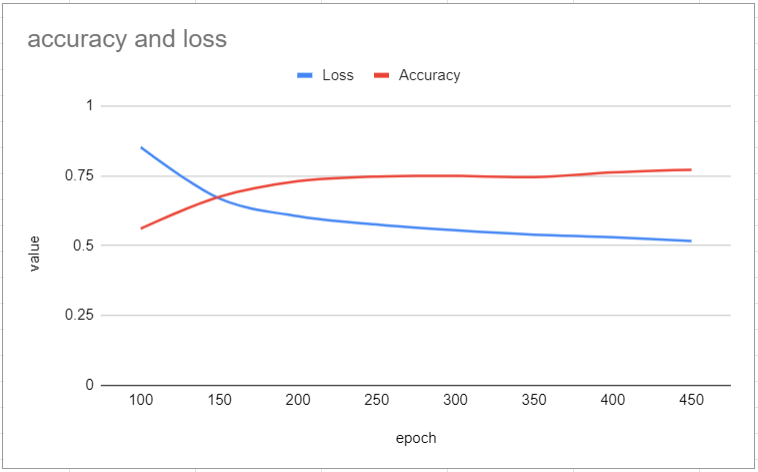
\includegraphics[width=0.48\textwidth]{accandloss.png}
    \caption{Loss value and Accuracy}
    \label{fig:accandloss}
\end{figure}
And an example of the recommendation system is shown in Figure 3. 
\begin{figure}[!htb]
    \centering
    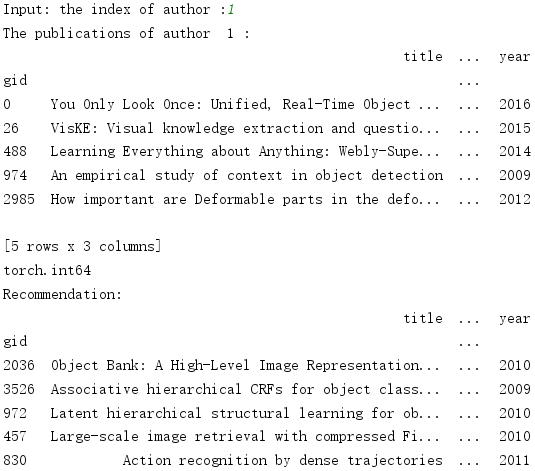
\includegraphics[width=0.48\textwidth]{demo.png}
    \caption{An example of the Recommendation System}
    \label{fig:demo}
\end{figure}
%\vspace{-1ex}
%%%%%%%%%%%%%%%%%%% Section 8 %%%%%%%%%%%%%%%%%%%%%%%
\section{Experiment 2}
\label{sec-expt}

Using real-world and synthetic dataset, we experimentally verify the efficiency and effectiveness of our LIGCN techniques.

\stitle{Datasets} We used one real-world graphs, that is \textbf{{\em DBpedia}} \footnote{\scriptsize\url{https://wiki.dbpedia.org/develop/datasets}}, a knowledge-based graph that contains a set of triples with size of $33,449,633$. We used a parser to further process this giant knowledge graph to a graph with $9595$ nodes and $5540$ edges.
Each node includes $4$ attributes and each edge reflects the ``influence" relationship.

We also employed \textbf{{\em BSBM}} \footnote{\scriptsize\url{http://wifo5-03.informatik.uni-mannheim.de/bizer/berlinsparqlbenchmark/}}
e-commerce benchmark to generate synthetic knowledge graphs over a set of products with different
types, related vendors and offers made by vendors. The generator is
controlled by the number of nodes (up to 60M), edges (up to
152M), and attribute labels drawn from an alphabet $\Sigma$ of $3080$ labels. We processed these synthetic knowledge graphs further to aggregate related attributes and generated a graph with two types of entities- product and offer. Different offers that are made by the same vendor are connected by edges and different offers for the same product are also connected. 

As there is no ground truth of erroneous entities in the above datasets, we need to inject errors into the attributed networks for our empirical evaluation. We refer to error generation tasks in {\em BART} \cite{arocena2015messing} to control the error-generation process. {\em BART} can generate constraint-induced errors with a set of configuration parameters , e.g. error percentage for each violation of the constraints in a systematic manner. At the same time, {\em BART} is capable to generate random errors of several kinds, e.g. typos, bogus or null values, and outliers. For instance, in the synthetic dataset, we organized product and offer entities respectively as two relation tables and manually construct a set of functional dependencies or conditional functional dependencies,  e.g. for products with the same product id in two tables, their product type should be the same. At the same time, we added some random errors into these two tables. Then, by comparing the difference between the clean and polluted tables and transferring them back to the graph organization, we got the ground truth labels.

\stitle{Compared Methods}. We compare the proposed \textbf {LIGCN} framework with the following popular and state-of-the-art erroneous entity detection methods:
(1) GCN \cite{kipf2016semi} jointly considers the node attributes and graph topology in the semi-supervised setting.
(2) GraphSAGE \cite{hamilton2017inductive} jointly considers the node attributes and graph topology but needs the supervised setting. In the experiment, we remove all the nodes without labels and their affiliated edges from the graph. We can treat GraphSAGE as a special form of GCN that implements node-wise sampling to get a fixed number of neighbors and also has the flexibility to select the aggregation function for node embedding.

\stitle{Metrics}
Metrics: Accuracy, F-1 score, precision.

We next present the details of our findings.




%%%%%%%%%%%%%%%%%%% Section 8 %%%%%%%%%%%%%%%%%%%%%%%
\section{Conclusions}
\label{sec-conclude}
In this project, we study a variant deep learning model GCN. We implement a file recommendation system based on traditional GCN model. To overcome shortcomings that are brought by the potential incompleteness of graphs, we also propose a new GCN based Model that can better capture the structure-aware representations that can be applied in the node classification task by inferring hidden links within graphs. We evaluate our proposed model on synthetic datasets and real-world datasets. We observe that infereing hideen links indeed can improve the performance of the erroneous entity classification tasks.

%-------------------------------------------------------------------------



{\small
%\bibliographystyle{ieee}
\setlength{\bibsep}{0pt}
\bibliographystyle{abbrvnat}
\bibliography{egbib}
}

\end{document}
